\section{Results\label{sec:results}}
  
  Benchmarking of a \gls{usp} implementation before and after the optimisations presented in the previous section have been applied, were collected using both a static diagnostic model and one representative of a physical particle simulation. All data presented was collected using an NVIDIA Titan-X (Pascal) in TCC mode with CUDA 8.0 on Windows 10.
  
  During each iteration the overall execution time in addition to separate timings for both the message emission and neighbourhood search stages are collected. However for the purposes of this research, the optimisations do not affect the construction of the \gls{usp} data structure, only the neighbourhood search timings are presented within this section.
  
  Where average neighbourhood volumes are referenced, these refer to the Moore neighbourhood volumes as opposed to the radial neighbourhood. During execution all messages within the Moore neighbourhood are loaded, even those that lie outside the radial neighbourhood which are not desired.
  \note{Could submit full data sets as a digital-only appendix}
  
  \subsection{Static Uniform Access}
    Under the diagnostic model, each thread is allocated a location. The location is both emitted as a message and used as the central point for a \gls{frnns} search. During the search the neighbour locations are averaged, this ensures both that optimisation has not removed necessary elements of the search and that we have a suitable export for validation between builds.
    
    Each benchmark configuration under the diagnostic model is executed for 100 iterations. The static model (such that each iteration was identical) combined with initial testing with higher iterations, showed runtimes to be highly stable. This permitted a reduction to 100 iterations, allowing a greater number of configurations to be executed within the parameter sweep, with negligible effect on the accuracy of the results.
  
    Two modes of initialisation have been used: uniform and uniform random. The uniform initialisation positions messages so that they are in an equally distributed grid. Whilst uniform initialisation ensures agents are strictly uniformly distributed through the environment, when the spacing of the environment is not a factor of the neighbourhood radius this can lead to uneven populations between bins. The uniform random initialisation utilises the CUDA device function \lstinline{float curand_uniform(curandState_t *)} to position messages within the environmental bounds, essentially producing a noisier version of the uniform random initialisation. To ensure consistency when using uniform random initialisation, the same seed value was used to initialise comparative benchmarks between builds.
    
    The diagnostic model has been carried out in both two and three dimensions, across a two dimensional parameter space collecting results from a total of 75,000 parameter combinations. Agent populations from 10,000 to 300,000 have been tested with average neighbourhood volumes from 17 to 430.
    \subsubsection{2D}
\begin{figure}[!t]
\centering
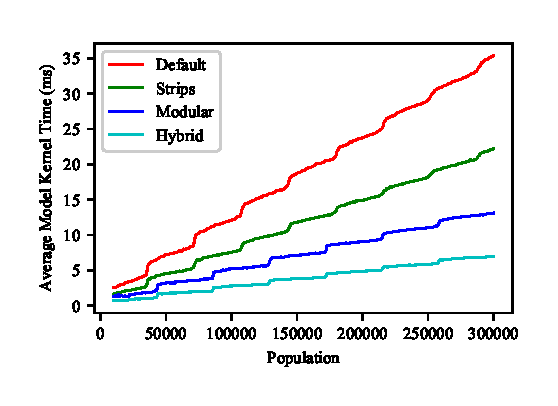
\includegraphics[width=\linewidth]{../resources/results/2d/22_neighbours.eps}
\caption{\label{fig:graph-2d-22neighbour-uniformrandom}A cross section from the uniform randomly initialised 2D parameter sweep of a two dimensional environment at a fixed density providing an average of 22 neighbours.}
\end{figure}
\begin{figure}[!t]
\centering
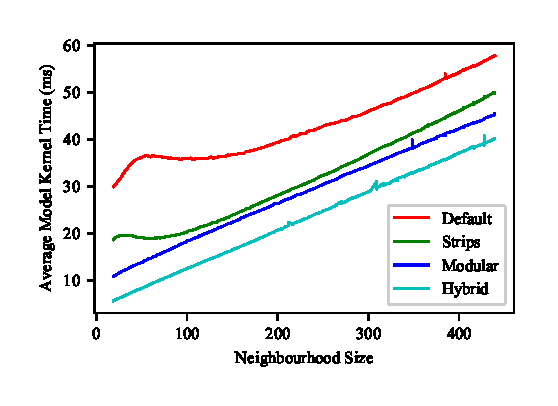
\includegraphics[width=\linewidth]{../resources/results/2d/257k_messages.eps}
\caption{\label{fig:graph-2d-257k message-uniformrandom}A cross section from the uniform randomly initialised 2D parameter sweep of a two dimensional environment at a fixed population of 257k messages.}
\end{figure}
      The parameter sweep of a two dimensional environment identified the peak proportional improvement as occurring with the configuration of 257,324 messages and an average of 22 neighbours with a uniform random initialisation. Figures \ref{fig:graph-2d-22neighbour-uniformrandom} and \ref{fig:graph-2d-257k message-uniformrandom} provide a cross-section of the parameter sweep about this configuration.
      
      The peak proportional improvement saw a 4.2 times speedup, with iterations under the Hybrid optimisation occurring in 11.6ms whereas the unoptimised implementation required 43.5ms per iteration. As the initial cross section of this result displayed evidence that even greater proportional and absolute improvement could be achieved with larger population size, an additional test extending the cross-section to a population size of \textit{TODO} was carried out.
      
      \note{Need to extend the 48 neighbour graph, but physical model been running all week (oops).}
      
      Most visible from Figure \ref{fig:graph-2d-22neighbour-uniformrandom} is that the Modular optimisation reduces the frequency of the recurring period in performance. This is evidence that Modular optimisation is improving hardware utilisation. This is similarly visible in the Hybrid optimisation but not under the Strips optimisation, suggesting the period is related to the change in hardware register usage in the Modular and Hybrid optimisations.
      
\begin{figure}[!t]
\centering
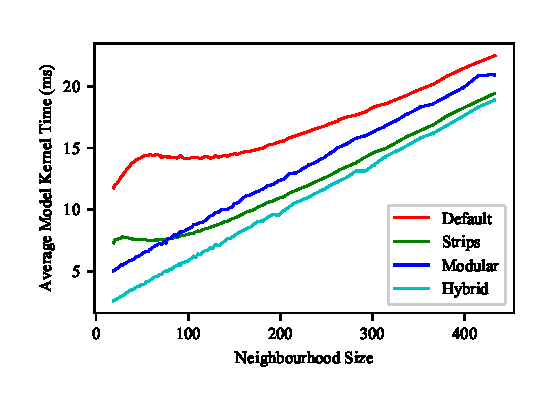
\includegraphics[width=\linewidth]{../resources/results/2d/100k_messages.eps}
\caption{\label{fig:graph-2d-100k message-uniformrandom}A cross section from the uniform randomly initialised 2D parameter sweep of a two dimensional environment at a fixed population of 100k messages.}
\end{figure}
      Whilst the results in Figure \ref{fig:graph-2d-257k message-uniformrandom} show a clear order of improvement per each optimisation technique. The previously discussed period visible in Figure \ref{fig:graph-2d-22neighbour-uniformrandom} changes with the population size. This leads to an alternate pattern of improvement at other population sizes. Figure \ref{fig:graph-2d-100k message-uniformrandom} shows this occurring with 100k messages, whereby the Strips optimisation provides a greater improvement than that of the Modular optimisation.

      Similar patterns can be seen in the results under uniform initialisation, however the peak proportional improvement of the Hybrid optimisation is 3.2 times speedup. Notably, when agents are strictly uniformly aligned, overall performance is in the order 2x faster. This presumably leads to better natural hardware utilisation. 
      
\begin{figure}[!t]
\centering
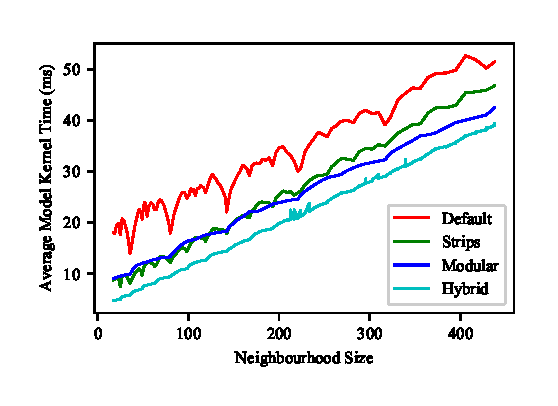
\includegraphics[width=\linewidth]{../resources/results/2d/256k_messages_uniform.eps}
\caption{\label{fig:graph-2d-256k message-uniform}A cross section from the uniformly initialised 2D parameter sweep of a two dimensional environment at a fixed population of 256k messages.}
\end{figure}
      Figure \ref{fig:graph-2d-256k message-uniform} shows the peak proportional improvement under uniform initialisation, whereby the Hybrid optimised implementation executed in an average of 6.7ms compared to the initial implementation executing in 21.7ms. In this configuration there were 256,354 agents with an average neighbourhood volume of 22.7. As previously discussed, the uniform initialisation results represent a noisier but faster instance of the uniform random initialisation.
      
      Across all of the 75,000 configurations tested under both uniform and uniform random initialisation, the Hybrid optimisation was the most performant in over 99\% of cases. In the remaining cases either Strips or Modular lead by a negligible margin, notably these occurrences primarily occurred at low population sizes with large neighbourhood volumes.
      
    \subsubsection{3D}
      When the same model is benchmarked in a three dimensional environment an even higher peak proportional improvement of 5.4x speedup from the Hybrid optimisation under uniform random initialisation is seen. This occurs with 40,000 agents with an average neighbourhood volume of 47.
      
\begin{figure}[!t]
\centering
\includegraphics[width=\linewidth]{../resources/results/3d/40k_messages.eps}
\caption{\label{fig:graph-3d-40kmessage-uniformrandom}A cross section from the uniform randomly initialised 2D parameter sweep of a three dimensional environment at a fixed population of 40k messages.}
\end{figure}
\begin{figure}[!t]
\centering
\includegraphics[width=\linewidth]{../resources/results/3d/47_neighbours.eps}
\caption{\label{fig:graph-3d-47neighbours-uniformrandom}A cross section from the uniform randomly initialised 2D parameter sweep of a three dimensional environment at a fixed  density providing an average of 47 neighbours.}
\end{figure}
      Figures \ref{fig:graph-3d-40kmessage-uniformrandom} and \ref{fig:graph-3d-47neighbours-uniformrandom} show cross-sectional graphs from the parameter sweep at the configuration of peak proportional improvement.
      
      It is clear that the three dimensional environment simply further emphasises the the difference in performance as seen in the earlier two dimensional results. Of note however, is that the visible period from the earlier Figure \ref{fig:graph-2d-22neighbour-uniformrandom} is far less pronounced in Figure \ref{fig:graph-3d-47neighbours-uniformrandom}. The period is  not clearly visible past 100,00 agents. This may be a result of device utilisation peaking much earlier with the larger Moore neighbourhoods found in three dimensional environments.

      As with two dimensional environment results, uniform initialisation saw a lesser peak proportional improvement. This occurred with 40,000 agents and a neighbourhood volume average of 73. Under this configuration the Hybrid optimisation executed in 4.34ms per iteration, whereas the pre-optimisation implementation executed in 18.3ms per iteration, equating to a 4.2 times speedup.
      
  \subsection{Physical model}
    The physical model used is an extension of that proposed by Chisholm et al as a means for benchmarking \gls{frnns} using a simple particle model analogue.\cite{CRM16} The extension modifies the force calculation to utilise sin as a means of smoothing. The addition of smoothing reduces the applied forces about the equilibrium position, such that the particle jitter about equilibrium position from the initial model is eliminated. Additionally this has made it possible to merge the attraction and repulsion parameters.
    
    The new force calculation formula therefore takes the form $F_{ij} = sin(-2\pi(\frac{d_{ij}}{r}))F$, whereby: $d_{ij}$ is the scalar distance between source particle $i$ and neighbour particle $j$, $r$ is the interaction radius and $F$ is the unified force dampening argument. $F_{ij}$ is subsequently multiplied by the normalised direction vector from $i$ to $j$. As with the original model, $F_{ij}$ is calculated for all neighbour particles with the sum of the resulting value providing the final offset that is applied to the source particle.
    
    This model differs from the prior diagnostic model, in that the particles (the message emitters), move slightly within the environment with each time step. Initially they start distributed in a pseudo uniform arrangement, and during runtime they move to create clusters of particles arranged in circles in two dimensions, and spheres in three dimensions. This has the effect of creating hotspots within the environment whereby neighbourhoods are very high volume and respectively dead zones with little no particles. This is a somewhat extreme instance of behaviour that can be observed in complex systems, such as pedestrian models whereby a bottle-neck in the environment creates a blockage.
    
    Each configuration is executed for 500 iterations, visual testing showed with the force modifier of $0.01$ this duration was required to consistently reach a steady state.
        
    \note{Included results are currently preliminary, taken from an incomplete parameter sweep. I seem to have miscalculated the requisite runtime. Should probably adjust and restart else we might be waiting a couple of weeks.}
    
\begin{figure}[!t]
\centering
\includegraphics[width=\linewidth]{../resources/results/2d/circles_10kmessage.eps}
\caption{\label{fig:graph-2d-circles-40kmessage}A cross section from the uniform randomly initialised 2D parameter sweep of the circles physical model benchmark in a two dimensional environment at a fixed population of 10k messages.}
\end{figure}

\begin{figure}[!t]
\centering
\includegraphics[width=\linewidth]{../resources/results/2d/circles_18-19_neighbours.eps}
\caption{\label{fig:graph-2d-circles-18-19neighbour}A cross section from the uniform randomly initialised 2D parameter sweep of the circles physical model benchmark in a two dimensional environment at a fixed population of 40k messages.}
\end{figure}
    In two dimensions the peak proportional improvement seen was 2.4x with a population size of 41,140 with neighbourhood volume starting at 18.7, increasing to 19.5 by completion. In this case the Hybrid optimisation executed each iteration of \gls{frnns} in 4.55ms whereas that lack the optimisation required 12.62ms. Figures \ref{fig:graph-2d-circles-40kmessage} and \ref{fig:graph-2d-circles-18-19neighbour} provide cross-sectional graphs of the parameter sweep about this point.
    
\begin{figure}[!t]
\centering
\includegraphics[width=\linewidth]{../resources/results/2d/circles_10kmessage.eps}
\caption{\label{fig:graph-2d-circles-10kmessage}A cross section from the uniform randomly initialised 2D parameter sweep of the circles physical model benchmark in a two dimensional environment at a fixed population of 10k messages.}
\end{figure}
    Notable of these results from the physical model parameter sweep, shown in Figure \ref{fig:graph-2d-circles-10kmessage}, is that in a proportion of cases the Hybrid and Modular optimisation negatively affected performance. The worst cases for both optimisations saw a population of 10,000 and average neighbourhoods of 192+. This lead the Hybrid and Modular performing at 0.88 and 0.54 times speed respectively. The worst case for strips was still an improvement of a mere 1.04 times speedup.
    
  \subsection{Concluding Analysis}
    These results have shown that whilst improvements as significant as 5x speedup are possible with pseudo-uniformly distributed messages, performance even with the optimisations presented in this paper struggle to provide even 3x speedup when messages are organised such that dense clusters exist. More research is required to classify the distributions found in complex systems, so that they can be better analysed for targeted optimisation.

